%\documentclass[draft]{ws-bme}
\documentclass{ws-bme}
\usepackage{multicol,balance}
\begin{document}

%\catchline{1}{1}{2006}{}{}
\markboth{Author's Name}{Paper Title}

\title{INSTRUCTIONS FOR TYPESETTING MANUSCRIPT\\
USING \LaTeX}

\author{First Author$^{*}$ and Second Author$^{\dag,\ddag}$}

\address{$^{*}\!$University Department, University Name, Address\\
City, State ZIP/Zone, Country,\\
\email{fauthor\_id@domain\_name} \\[6pt]
$^{\ddag}\!$Group, Company, Address\\
City, State ZIP/Zone, Country\\
\email{sauthor\_id@domain\_name}}

\maketitle

\begin{history}
\received{Day Month Year}
\revised{Day Month Year}
\end{history}

\footnotetext{$^{\ddag}$Corresponding author: Prof. Second Author,
University Department, University Name, Address,
City, State ZIP/Zone, Country. Tel.: +000-0-0000000, ext 000; Fax:
+000-0-0000000; E-mail: sauthor\_id@domain\_name.}

\begin{abstract}
The abstract should summarize the context,
content and conclusions of the paper. It should not contain any
references or displayed equations. Typeset the abstract in 8~pt
Times Roman with baselineskip of 10~pt, making an indentation of
.65in on the left and right margins.
\end{abstract}

\keywords{A list of 3--5 keywords are to be supplied.}

\vspace*{-1.5pc}

\begin{multicols}{2}
\section*{THE MAIN TEXT}
Contributions are to be in English. Authors are
encouraged to have their contribution checked for grammar.
American spelling should be used. Abbreviations are allowed but
should be spelt out in full when first used. Integers ten and
below are to be spelt out. Italicize foreign language phrases
(e.g.,~Latin, French).

For the title, try
not to use more than three lines. Typeset the title in 14~pt Times
Roman, uppercase and boldface. Typeset author names in 12~pt Times Roman.
Use the footnote to indicate the present or permanent address of
the author. Affiliations are typeset in 11~pt Times italics. State completely without
abbreviations the affiliation and mailing address, including
country.

The text is to be typeset in 10~pt Times \hbox{Roman},
single-spaced with baselineskip of 13~pt. Text area is 6.9~in across and 9.3~in deep (including running
title). Final pagination and insertion of running titles will be
done by the publisher.

\section*{SECTION HEADINGS}
Section headings should be typeset in boldface, with all the
letters capitalized.

\subsection*{Subheadings}
Subheadings should be typeset in boldface, with the
first letter of the first word capitalized.

\subsubsection*{Sub-subheadings}
Typeset in italics and
capitalize the first letter of the first word only.

\subsection*{Numbering and spacing}
Sections, subsections and sub-subsections are all unnumbered.
Unnumbered sections can be obtained by using \verb|\section*|, \verb|\subsection*| and \verb|\subsubsection*| commands.
Use double spacing before major and subheadings, and single spacing\break after sub-subheadings.

\section*{LISTS OF ITEMS}
Lists are broadly classified into four major categories that can
randomly be used as desired by the author:
\begin{alphlist}[(d)]
\item Numbered list.
\item Lettered list.
\item Unnumbered list.
\item Bulleted list.
\end{alphlist}

\subsection*{Numbered and lettered list}

\begin{enumerate}
\item[] The \verb|\begin{arabiclist}[]| command is used for the arabic
number list (arabic numbers appearing within parenthesis), e.g., (1),
(2), etc.

\smallskip

\item[] The \verb|\begin{romanlist}[]| command is used for the roman
number list (roman numbers appearing within parenthesis), e.g., (i),
(ii), etc.

\smallskip

\item[] The \verb|\begin{Romanlist}[]| command is used for the cap roman
\hbox{number list} (cap roman numbers appearing within parenthesis),
e.g., (I), (II), etc.

\smallskip

\item[] The \verb|\begin{alphlist}[]| command is used for the alphabetic
list (alphabets appearing within parenthesis), e.g., (a), (b), etc.

\smallskip

\item[] The \verb|\begin{Alphlist}[]| command is used for the cap
alphabetic list (cap alphabets appearing within parenthesis), e.g.,
(A), (B), etc.
\end{enumerate}
Note: For all the above mentioned lists (with the exception of
alphabetic list), it is obligatory to enter the last entry's number
in the list within the square bracket, to enable unit alignment.

\subsection*{Bulleted and unnumbered list}

\begin{enumerate}
\item[] The \verb|\begin{itemlist}| command is used for the bulleted list.

\smallskip

\item[] The \verb|\begin{unnumlist}| command is used for creating the
  unnumbered list with the turnovers hangindent by 1\,pica.
\end{enumerate}

Lists may be laid out with each item marked by a dot:
\begin{itemlist}
\item item one
\item item two.
\end{itemlist}

Items may also be numbered with lowercase\break Arabic numerals:
\begin{arabiclist}[(2)]
\item item one
\item item two
    \begin{alphlist}[(a)]
    \item lists within lists can be numbered with lowercase Roman letters
    \item second item.
    \end{alphlist}
\end{arabiclist}

\section*{FOOTNOTES}
Footnotes should be numbered sequentially in superscript lowercase
Roman letters.\footnote{Footnotes should be typeset in 9~pt Times Roman at the bottom of the page.}

\section*{MATHEMATICAL FORMULAE}
\paragraph{Inline:}
For in-line formulae use \verb|\( ... \)| or \verb|$ ... $|. Avoid
built-up constructions, for example fractions and matrices, in
in-line formulae. Fractions in inline can be typed with a solidus, e.g., \verb|x+y/z=0|.

\paragraph{Display:}
Displayed equations should be numbered consecutively in
the paper, with the number set flush right and enclosed in
parentheses. For numbered display formulae, use the displaymath
environment:

\verb|\begin{equation} ...| \verb|\end{equation}|.

For unnumbered display formulae, use
\verb|\[ ... \]|. For numbered displayed,
one-line formulae always use the equation environment. Do not use
\verb|$$ ... $$|. For example, the input for

\begin{equation}
\mu(n, t) = \frac{\sum\limits^\infty_{i=1}1
(d_i < t, N(d_i) = n)}
{\int\limits^t_{\sigma=0}1(N(\sigma)=n)d\sigma}
\label{eq1}
\end{equation}

\noindent is:

\begin{verbatim}
\begin{equation}
\mu(n, t) = \frac{\sum\limits^\infty_{i=1}1
(d_i < t, N(d_i) = n)}
{\int\limits^t_{\sigma=0}1
(N(\sigma)=n)d\sigma}
\label{eq1}
\end{equation}
\end{verbatim}

For displayed multi-line formulae, use the \verb|eqnarray| environment. For example,

\begin{verbatim}
\begin{eqnarray}
\zeta\mapsto\hat{\zeta}&=&a\zeta+b\eta\,,\\
\eta\mapsto\hat{\eta}&=&c\zeta+d\eta\,.
\label{eq2n3}
\end{eqnarray}
\end{verbatim}

\noindent produces:
\begin{eqnarray}
\zeta\mapsto\hat{\zeta}&=&a\zeta+b\eta\,,\\
\eta\mapsto\hat{\eta}&=&c\zeta+d\eta\,.
\label{eq2n3}
\end{eqnarray}

\LaTeX\ does not break long equations to make them fit within the
margins as it does with normal text. It is therefore up to you to
format the equation appropriately (if they overrun the margin.) This
typically requires some creative use of an eqnarray to get elements
shifted to a new line and to align nicely, e.g.,

\begin{eqnarray}
\left(1+x\right)^n &=& 1 + nx + \frac{n\left(n-1\right)}{2!}x^2 \nonumber\\
  & & + \frac{n\left(n-1\right)\left(n-2\right)}{3!}x^3 \nonumber\\
  & & + \frac{n\left(n-1\right)\left(n-2\right)\left(n-3\right)}{4!}x^4 \nonumber\\
  & & + \ldots n{\rm th}.
\end{eqnarray}

Superscripts and subscripts that are words or abbreviations, as in
\( \pi_{\mathrm{low}} \), should be typed as roman letters;
this is done as \verb|\( \pi_{\mathrm{low}} \)|
instead of \( \pi_{low} \) done with \verb|\( \pi_{low} \)|

For geometric functions, e.g.,~exp, sin, cos, tan, etc., please use the macros
\verb|\sin, \cos, \tan|. These macros give proper spacing in mathematical formulae.

It is also possible to use the \AmS-\LaTeX{}
package, which can be obtained from the \AmS\ and various \TeX{}
archives.

Equations should be referred to in abbreviated form,
e.g.,~``Eq.~(\ref{eq1})'' or ``(2)''. In multiple-line equations,
the number should be given on the last line.

Displayed equations are to be centered on the page width. Standard
English letters like x are to appear as $x$ (italicized) in the
text if they are used as mathematical symbols. Punctuation marks
are used at the end of equations as if they appeared directly in
the text.

\section*{THEOREMS AND DEFINITIONS}
\LaTeX{} provides \verb|\newtheorem| to create new theorem
environments. The WSPC document styles contain a set of pre-defined
environments for theorems, definitions, proofs, remarks, etc., e.g.,
\begin{verbatim}
\begin{theorem}[Longo, 1998]
For a given $Q$-system...
\[
N = \{x \in N; T x = \gamma (x) T, T x^* =
\gamma (x^*) T\}\,,
\]
and $E_\Xi (\cdot) = T^* \gamma (\cdot) T$
gives a conditional expectation onto $N$
\end{theorem}
\end{verbatim}

\noindent generates

\begin{theorem}[Longo, 1998]
For a given $Q$-system...
\[
N = \{x \in N; T x = \gamma (x) T, T x^* = \gamma (x^*) T\}\,,
\]
and $E_\Xi (\cdot) = T^* \gamma (\cdot) T$ gives a conditional
expectation onto $N$
\end{theorem}

\noindent and

\begin{verbatim}
\begin{theorem}
We have $\# H^2 (M \supset N) < \infty$ ...
\end{theorem}
\end{verbatim}

\noindent produces

\begin{theorem}
We have $\# H^2 (M \supset N) < \infty$ for an inclusion $M \supset
N$ of factors of finite index.
\end{theorem}

To add a new theorem-type environments to an article, use

\begin{verbatim}
\newtheorem{example}{Example}[section]

\let\Examplefont\upshape
\def\Exampleheadfont{\bfseries}
\end{verbatim}

\section*{FLOATS}
\subsection*{Tables}
Put tables and figures in text using the table and figure environments,
and position them near the first reference of the table or figure in
the text. Please avoid long captions in figures and tables.

\paragraph{Input:}

\begin{verbatim}
\begin{tablehere}
\tbl{... table caption ...}
{\begin{tabular}{@{}lcccr@{}}
\toprule
ID & $m$ & $R^2$ & $x_2$ & Times (s)\\
\colrule
11 & 100 & 3135 & 1138 & $<98$\\
...
15 & 100 & 3135 & 1138 & $<102$\\
\botrule
\end{tabular}}
\label{tbl1}
\end{tablehere}
\end{verbatim}

\noindent {\bf Output:}

\begin{tablehere}%[H]
\tbl{... table caption ...}
{\begin{tabular}{@{}lcccr@{}}
\toprule
ID & $m$ & $R^2$ & $x_2$ & Times (s)\\ \colrule
11 & 100 & 3135 & 1138 & $<98$\\
12 & 100 & 3135 & 1138 & $<99$\\
13 & 100 & 3135 & 1138 & $<100$\\
14 & 100 & 3135 & 1138 & $<101$\\
15 & 100 & 3135 & 1138 & $<102$\\ \botrule
\end{tabular}}\label{tab:smtab}
\end{tablehere}

By using \verb|\tbl| command in table environment, long captions will be justified to the table width while the short or single line captions are centered.
\verb|\tbl{table caption}{tabullar environment}|.

For most tables, the horizontal rules are obtained by:

\begin{tabular}{ll}
{\bf toprule} & one rule at the top\\
{\bf colrule}& one rule separating column heads\\ & from data cells\\
{\bf botrule}& one bottom rule\\
{\bf Hline} & one thick rule at the top and\\ & bottom of the tables with multiple\\& column heads\\
\end{tabular}

To avoid the rules sticking out at either end
of the table, add \verb|@{}| before the first and after the last descriptors, e.g., {@{}llll@{}}. Please avoid vertical rules in tables.
But if you think the vertical rule is a must,
you can use the standard \LaTeX{} \verb|tabular| environment.

Tables should have a uniform style throughout the
contribution. It does not matter how you place the
inner lines of the table, but we would prefer the border lines to be
of the style as shown in our sample tables.
For the inner lines of the table, it looks better
if they are kept to a minimum.

If tables need to extend over to a second page, the continuation
of the table should be preceded by a caption, e.g.,~``Table~1 ({\it
Continued})''.

\subsection*{Figures}
A figure is obtained with the following commands

\begin{verbatim}
\begin{figurehere}
\centerline{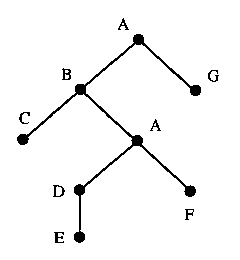
\psfig{file=bmef1.eps,
                             width=3.2cm}}
\caption{...caption here...} \label{fig1}
\end{figurehere}
\end{verbatim}

\begin{figurehere}
\centerline{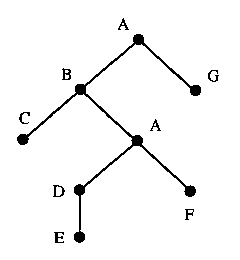
\psfig{file=bmef1.eps,width=3.2cm}}
\caption{ ... caption here ... }
\label{fig1}
\end{figurehere}

Figures are to be inserted in the text nearest their
first reference. Original Indian ink drawings of glossy prints are
preferred. Please send one set of originals with copies. If the
publisher is required to reduce the figures, ensure that the
figures (including lettering and numbers) are large enough to be
clearly seen after reduction.

Figures are to be sequentially numbered with\break Arabic
numerals. The caption must be placed below the figure. For those
figures with multiple parts which appear on different pages, it is
best to place the full caption below the first part, and have
e.g.,~``Fig.~1 ({\it Continued})'' below the last part.

Previously published material must be accompanied by written
permission from the author and publisher.

The preferred graphics formats are TIF and Encapsulated PostScript
(EPS) for any type of image. Our \TeX\ installation requires EPS,
but we can easily convert TIF to EPS. Many other formats, e.g., PICT
(Macintosh), WMF (Windows) and various proprietary formats, are not
suitable. Even if we can read such files, there is no guarantee that
they will look the same on our systems as on yours.

Adjust the scaling of the figure until it is correctly positioned,
and remove the declarations of the lines and any anomalous spacing.

\begin{table*}
\tbl{Comparison of acoustic for frequencies for piston-cylinder problem.}
{\begin{tabular}{@{}cccc@{}} \toprule
& Analytical frequency & TRIA6-$S_1$ model &  \\
Piston mass & (Rad/s) & (Rad/s) & \% Error$^{\text a}$ \\ \colrule
1.0\hphantom{00} & \hphantom{0}281.0 & \hphantom{0}280.81 & 0.07 \\
0.1\hphantom{00} & \hphantom{0}876.0 & \hphantom{0}875.74 & 0.03 \\
0.01\hphantom{0} & 2441.0 & 2441.0\hphantom{0} & 0.0\hphantom{0} \\
0.001 & 4130.0 & 4129.3\hphantom{0} & 0.16\\ \botrule
\end{tabular}
}
\begin{tabnote}
$^{\text a}$ Sample table footnote.\\
\end{tabnote}
\label{tbl2}
\end{table*}

\begin{figure*}
\begin{center}
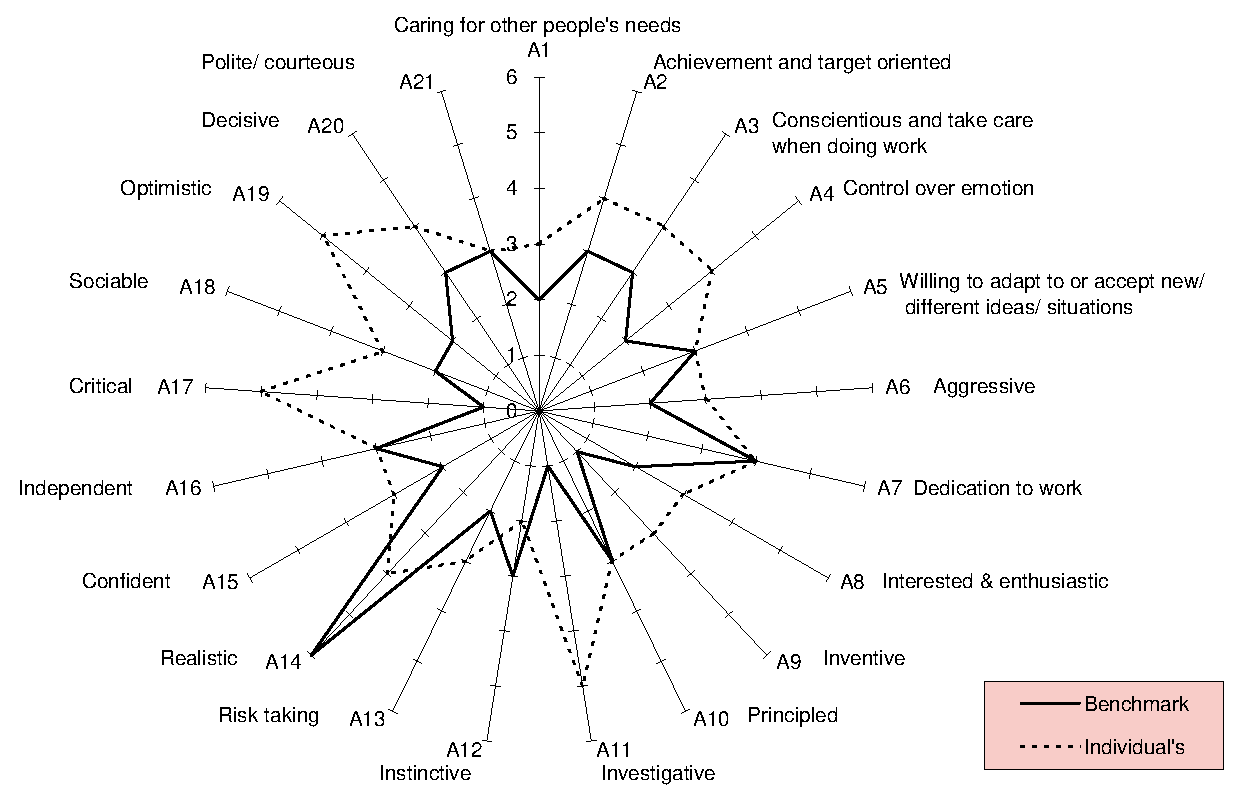
\psfig{file=bmef2.eps,width=6in}
\end{center}
\caption{The bifurcating response curves of system
$\alpha=0.5$, $\beta=1.8$, $\delta=0.2$, $\gamma=0$: (a)
$\mu=-1.3$ and (b) $\mu=0.3$.}
\label{fig2}
\end{figure*}

We recommend the use of single column-wide tables and figures wherever
possible. Tables and \hbox{figures} spanning two columns can be typeset
with the following environments:

\begin{itemlist}
\item \verb|table*| and
\item \verb|figure*|.
\end{itemlist}

\noindent {\bf Example:}\\[-3pt]

\noindent {\it Table:}
\begin{verbatim}
\begin{table*}
\tbl{Comparison of ...}
{\begin{tabular}{@{}cccc@{}} \toprule
Piston mass & Analytical ...\\ \colrule
1.0... \\
0.001... \\ \botrule
\end{tabular}}
\begin{tabnote}
$^{\text a}$ Sample table footnote.\\
\end{tabnote} \label{tbl2}
\end{table*}
\end{verbatim}

\noindent {\it Figure:}
\begin{verbatim}
\begin{figure*}
\begin{center}
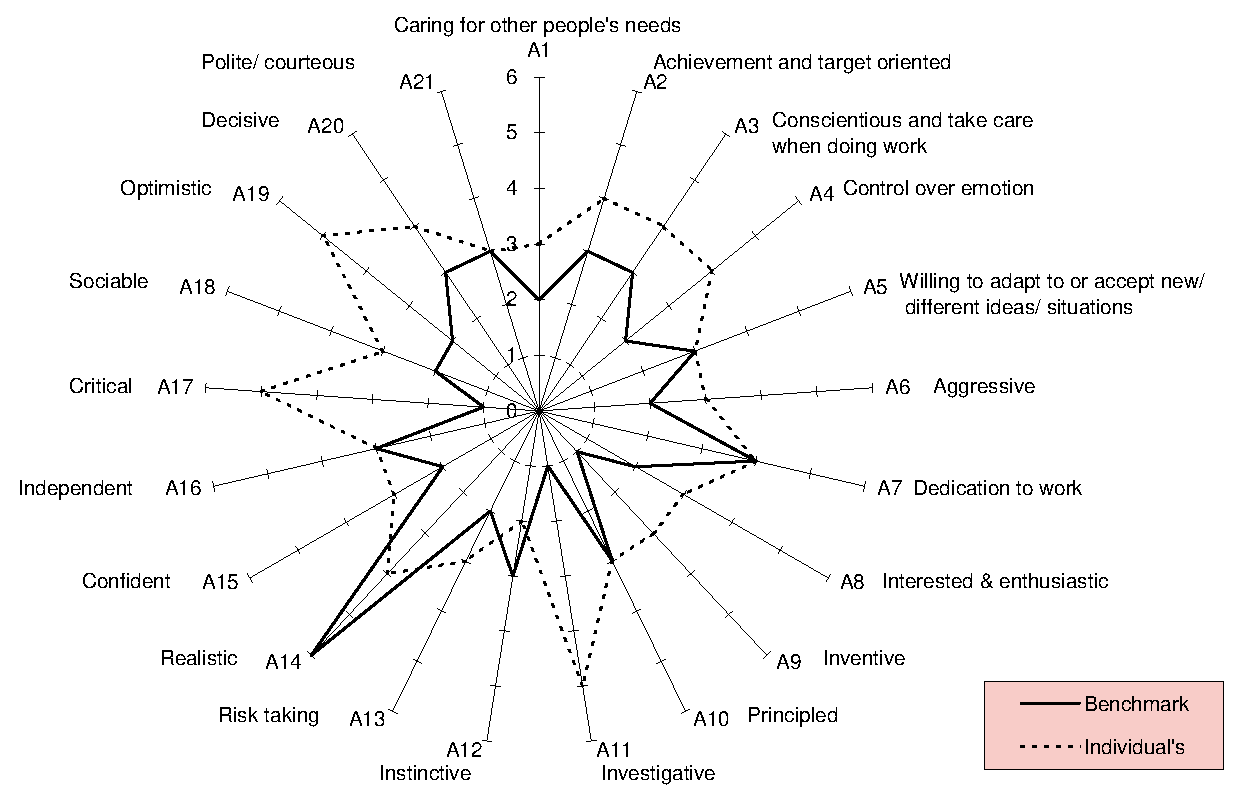
\psfig{file=bmef2.eps,width=6in}
\end{center}
\caption{The bifurcating response ...}
\label{fig2}
\end{figure*}
\end{verbatim}

\begin{sidewaystable*}
\tbl{Positive values of $X_0$ by eliminating $Q_0$ from
Eqs.~(15) and (16) for different values of the parameters $f_0$,
$\lambda_0$ and $\alpha_0$ in various dimension.}
{\begin{tabular}{@{}ccccccccccc@{}}
\toprule\\[-8pt]
{} &  & &\multicolumn{8}{c}{Positive roots ($X_0$)}\\[3pt]
\cline{4-11}\\[-6pt]
$f_0$ & $\lambda_0$ & $\alpha_0$ &4D &5D &6D &7D &8D &10D &12D &16D\\[3.5pt]
\hline\\[-6pt]
$-0.033$ &0.034 &0.1
&6.75507, &4.32936, &3.15991, &2.44524,
&1.92883, &0.669541, &--- &---\\[3.5pt]
&&&1.14476 &1.16321 &1.1879
&1.22434 &1.29065
&0.415056\\[7pt]
$-0.1$ &0.333 &0.2
&3.15662, &1.72737, &--- &--- &--- &--- &--- &---\\[3.5pt]
&&&1.24003 &1.48602\\[7pt]
$-0.301$ &0.302 &0.001
&2.07773, &--- &--- &--- &--- &--- &--- &---\\[3.5pt]
&&&1.65625\\[7pt]
$-0.5$ &0.51 &0.001
&--- &--- &--- &--- &--- &--- &--- &---\\[7pt]
0.1 &0.1
&2&1.667, &1.1946
&--- &--- &--- &--- &--- &---\\[3.5pt]
&&&0.806578 &0.858211\\[7pt]
0.1 &0.1 &10
&0.463679 &0.465426 &0.466489 &0.466499
&0.464947 &0.45438 &0.429651 &0.35278\\[7pt]
0.1 &1
&0.2
&--- &--- &--- &--- &--- &--- &--- &---\\[7pt]
0.1 &5
&5&--- &--- &--- &--- &--- &--- &--- &---\\[7pt]
1 &0.001 &2
&0.996033, &0.968869, &0.91379, &0.848544,&0.783787, &0.669541,
&0.577489, &---\\[3.5pt]
&&&0.414324 &0.41436 &0.414412 &0.414489 &0.414605
&0.415056 &0.416214\\[7pt]
&0.001 &0.2
&0.316014, &0.309739, &--- &--- &--- &--- &--- &---\\[3.5pt]
&&&0.275327 &0.275856\\[7pt]
&0.1
&5
&0.089435 &0.089441 &0.089435 &0.089409 &0.08935
&0.089061 &0.088347 &0.084352\\[7pt]
&1 &3&0.128192 &0.128966 &0.19718, &0.169063, &0.142103,
&--- &--- &---\\[3.5pt]
&&&& &0.41436 &0.414412 &0.414489\\[3pt]
\Hline
\end{tabular}}\label{tbl3}
\end{sidewaystable*}

Very large figures and tables should be placed on a separate page
by themselves. Landscape tables and figures can be typeset with the following environments:

\begin{itemlist}
\item \verb|sidewaystable| and
\item \verb|sidewaysfigure|.
\end{itemlist}

\noindent {\bf Example:}

\begin{verbatim}
\begin{sidewaystable*}
\tbl{Positive values of ...}
{\begin{tabular}{@{}ccccccccccc@{}}
...
\end{tabular}}
\label{tbl3}
\end{sidewaystable*}
\end{verbatim}

\section*{CITATIONS}
We have used \verb|\bibitem| to produce the bibliography. Citations
in the text use the labels defined in the bibitem declaration, e.g.,
the first paper by Golub\cite{shi92} is cited using the command
\verb|\cite{shi92}|. Bibitem labels should be unique.

For multiple citations, do not use \verb|\cite{1}|, \verb|\cite{2}|, but use
\verb|\cite{1,2}| instead.

When the reference forms part of the sentence, it should not be
typed in superscripts, e.g.,

\begin{itemlist}
\item ``One can show from Ref.~\refcite{kol88} that $\ldots$'',\break
\item ``See Refs.~\refcite{baj94} and \refcite{bog87} for more details.''
\end{itemlist}

This is done using the LaTeX command: ``\verb|Ref.~\refcite{name}|''.

\section*{NOTE ADDED}
A note can be added before Acknowledgments.

\section*{ACKNOWLEDGMENTS}
This part should come before References.
Funding information may also be included here.

\setcounter{equation}{0}
\renewcommand{\theequation}{A.\arabic{equation}}
\section*{APPENDICES}
\noindent Appendices should be used only
when absolutely necessary. They should come immediately before
References. If there is more than one appendix, number them
alphabetically. Number displayed equations occurring in the
appendix as (\ref{aeqn1}), (A.2), etc.:
\begin{equation}
\mu(n, t) = \frac{\sum\limits^\infty_{i=1} 1(d_i < t, N(d_i) = n)}
{\int\limits^t_{\sigma=0} 1(N(\sigma) = n)d\sigma}\,\,
.\label{aeqn1}
\end{equation}

\section*{REFERENCES}
Article titles should be stated in full but standard abbreviations
should be used for journal names. Typeset reference in 9~pt Times
Roman, single spaced with baselineskip of 11 pt.

\subsection*{Examples}

\subsubsection*{Journal reference:}

\hangindent=1.12em Shieh MJ, Wong JM ,Wang CY, Basic principle and
clinical application of bipolar electrosurgical polypectomy snare,
{\it Biomed Eng Appl Basis Comm} {\bf 4}:123, 1992.

\noindent\hangindent=1.12em Kolenbramder KD, Dykstra CE, Lisy JM,
Torsional vibrational modes of (HF)3: IR-IR double resonance
spectroscopy and electrical interaction theory, {\it J Chem Phys}
{\bf 88}:5995, 1988.

\subsubsection*{Book reference:}

\hangindent=1.12em Bajpai PK, in Zhang X, Ikada Y (eds.) {\it
Biomedical materials research in the Far East (I)}, Kobunshi
Kankokai Inc, Kyoto, Japan, pp. 41--42, 1994.

\noindent\hangindent=1.12em Boger DL, Weinreb SN, {\it Hetero
Diels-Alder Methodology in Organic Synthesis}, Academic Press, San
Diego, 1987.

\begin{thebibliography}{9}
\bibitem{shi92} Shieh MJ, Wong JM ,Wang CY, Basic principle and clinical
application of bipolar electrosurgical polypectomy snare, {\it
Biomed Eng Appl Basis Comm} {\bf 4}:123, 1992.

\bibitem{kol88} Kolenbramder KD, Dykstra CE, Lisy JM, Torsional vibrational modes
of (HF)3: IR-IR double resonance spectroscopy and electrical
interaction theory, {\it J Chem Phys} {\bf 88}:5995, 1988.

\bibitem{baj94} Bajpai PK, in Zhang X, Ikada Y (eds.) {\it Biomedical materials
research in the Far East (I)}, Kobunshi Kankokai Inc, Kyoto, Japan,
pp. 41--42, 1994.

\bibitem{bog87} Boger DL, Weinreb SN, {\it Hetero Diels-Alder Methodology in
Organic Synthesis}, Academic Press, San Diego, 1987.
\end{thebibliography}
\end{multicols}
\end{document}
